\chapter{Análisis de los resultados}
\label{chap:Resultados}
\Abstract{En este capítulo se llevará a cabo una comparativo de todos los métodos creados para la detección de piezas así como los creados para la estimación de la orientación de piezas. Se realizará un estudio de precisión, robustez y rapidez de los sistemas creados.}
\section{Análisis de la segmentación}
Como ya se ha mencionado, se han desarrollado múltiples métodos para llevar a cabo el proceso de segmentación. Y todos tienen sus ventajas y desventajas y es importante conocerlas para así poder seleccionar que método o combinación de métodos emplear para la implantación con el brazo robótico. Es por ello que a continuación se van a comparar estos métodos tanto en precisión y tasa de fallos como en velocidad. Para ello se van a usar los resultados ya mostrados en este documento al desarrollar cada uno de estos métodos.

\subsection{Precisión, Exhaustividad, Tasa de fallos y FPPI}
Si se analizan los resultados se pueden observar dos patrones:
\begin{itemize}
\item Segmentación por color: Al comparar los resultados de este método frente a las redes neuronales se muestra la superioridad de estas. Este método solo puede competir al detectar piezas amarillas y esto es debido a que en las fotos analizadas no hay ningún otro objeto de color amarillo.
\item AlexNet y VGG-16: al comparar estas redes en igualdad de condiciones se observa claramente la superioridad de VGG-16. Al tratarse de una red más compleja es capaz de aprender más y por ello ha dado mejores resultados siempre que ha podido ser entrenada.
\end{itemize}

Si nos centramos solo en las redes neuronales, también se pueden extraer múltiples conclusiones:
\begin{itemize}
\item R-CNN: Destaca por ser uno de los métodos más precisos y seguros, solamente es superado por YOLO basado en VGG-16. Al hacer una comparativa justa frente al resto de métodos basados también en LEGONet se puede apreciar el verdadero potencial de R-CNN. Se trata de un método muy capaz, aunque muy poco eficiente.
\item Faster R-CNN: Se trata de una variante de R-CNN cuyo objetivo es mejorar la eficiencia del mismo reduciendo bastante el procesado, pero al hacerlo también pierde en capacidades. Ambas redes del tipo Faster R-CNN pierden frente a R-CNN basado en LEGONet pero a cambio son bastante más eficientes. Se puede observar en ellas la diferencia entre AlexNet y VGG-16 ya que esta segunda ha dado resultados mucho más positivos y se han aproximado bastante a R-CNN basado en AlexNet.
\item YOLO: Este tipo de redes se caracterizan por dar buenos resultados con un entrenamiento muy rápido además de ser bastante eficientes. Al analizar los resultados podemos ver que esto es cierto, las redes han aprendido rápidamente y siendo muy eficientes consiguen dar muy buenos resultados. Aun así, se puede observar que R-CNN basado en LEGONet es superior a YOLO basado en LEGONet aunque queda por detrás de YOLO basado en VGG-16. Esto muestra la superioridad de R-CNN al detectar piezas y la superioridad de VGG-16 frente a AlexNet.
\end{itemize}


\begin{figure}[ht]  %Estudio Amarillo
\vspace{-30pt}
  \subfloat{
	\begin{minipage}[c][1\width]{0.49\textwidth}
	   \centering
	   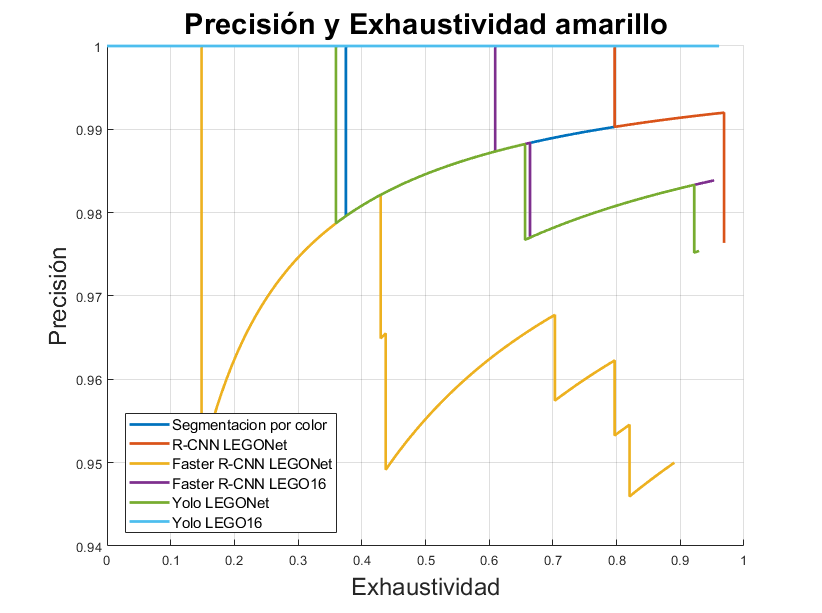
\includegraphics[width=1\textwidth]{Resultados/precision yellow.png}
	\end{minipage}}
  \hfill	
  \subfloat{
	\begin{minipage}[c][1\width]{0.49\textwidth}
	   \centering
	   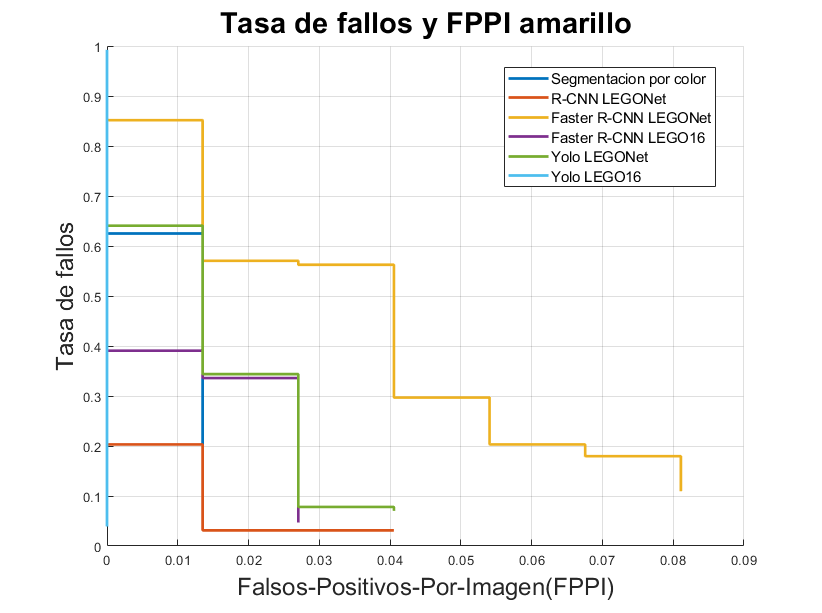
\includegraphics[width=1\textwidth]{Resultados/miss yellow.png}
	\end{minipage}}
\caption{Comparativa de los métodos de segmentación al detectar piezas amarillas}
\label{fig:yellow resultados}
\vspace{-5pt}
\end{figure}

\begin{figure}[ht]  %Estudio Rojo
\vspace{-30pt}
  \subfloat{
	\begin{minipage}[c][1\width]{0.49\textwidth}
	   \centering
	   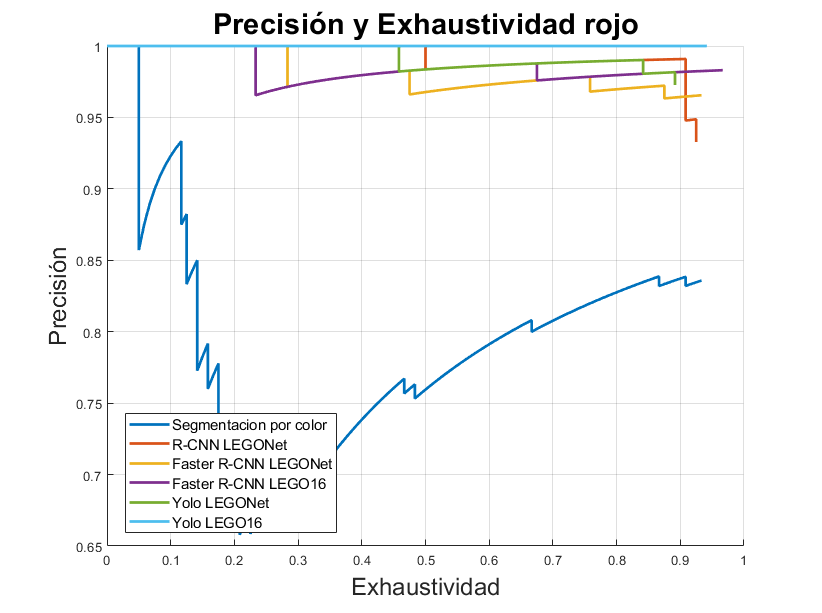
\includegraphics[width=1\textwidth]{Resultados/precision red.png}
	\end{minipage}}
  \hfill	
  \subfloat{
	\begin{minipage}[c][1\width]{0.49\textwidth}
	   \centering
	   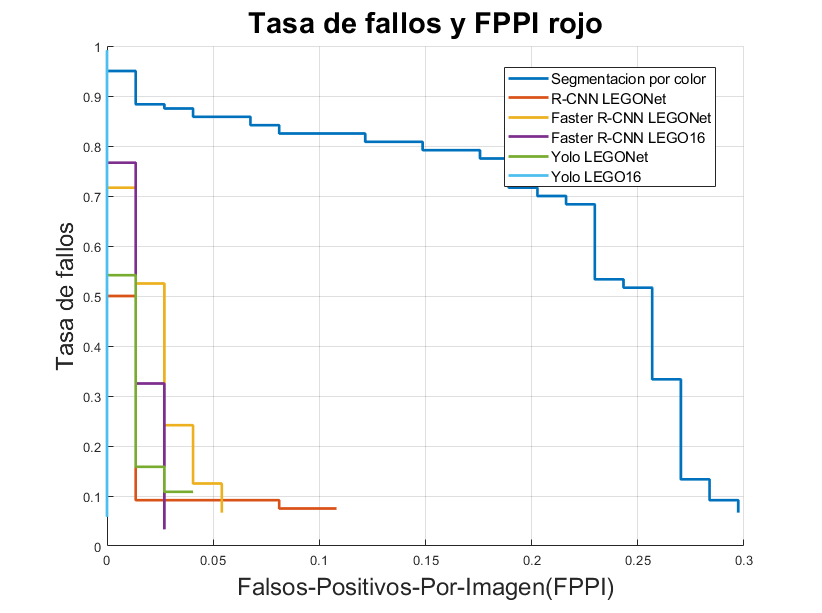
\includegraphics[width=1\textwidth]{Resultados/miss red.png}
	\end{minipage}}
\caption{Comparativa de los métodos de segmentación al detectar piezas rojas}
\label{fig:red resultados}
\vspace{-5pt}
\end{figure}

\begin{figure}[ht]  %Estudio Azul
\vspace{-30pt}
  \subfloat{
	\begin{minipage}[c][1\width]{0.49\textwidth}
	   \centering
	   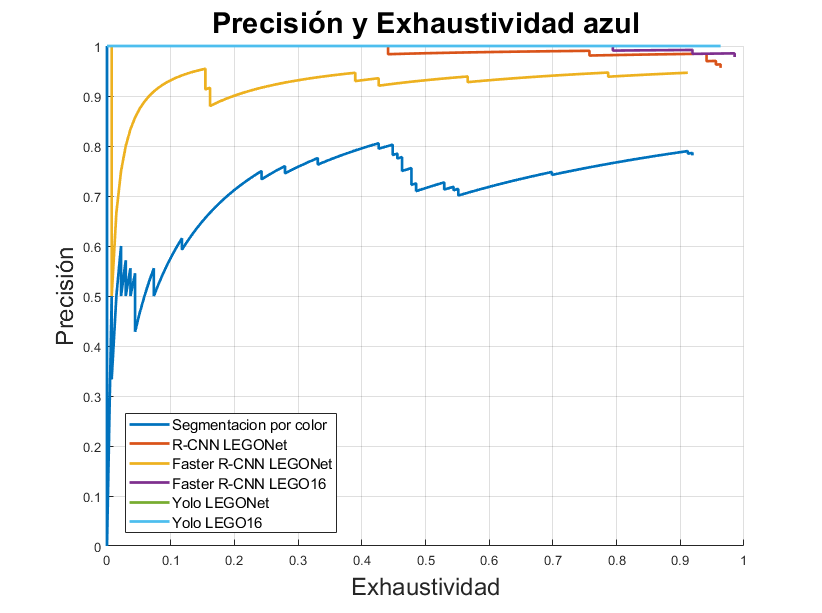
\includegraphics[width=1\textwidth]{Resultados/precision blue.png}
	\end{minipage}}
  \hfill	
  \subfloat{
	\begin{minipage}[c][1\width]{0.49\textwidth}
	   \centering
	   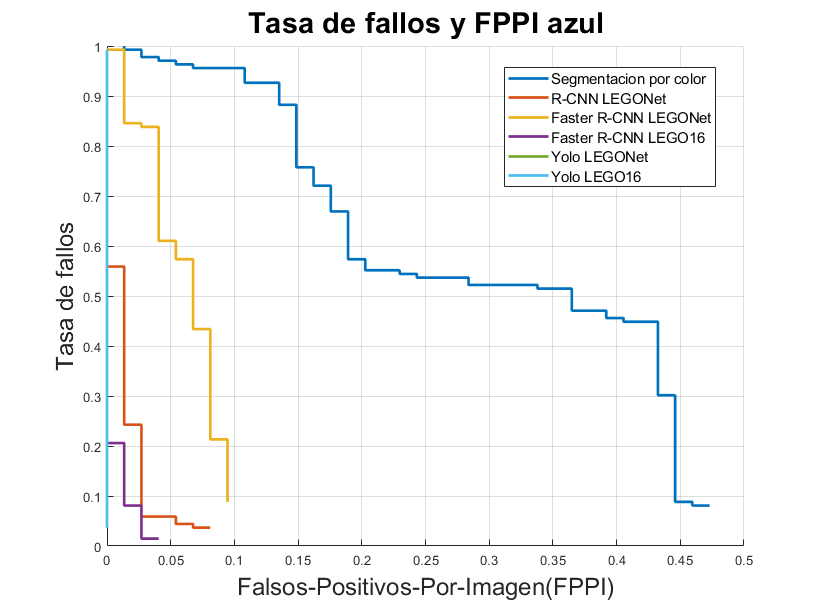
\includegraphics[width=1\textwidth]{Resultados/miss blue.png}
	\end{minipage}}
\caption{Comparativa de los métodos de segmentación al detectar piezas azules}
\label{fig:blue resultados}
\vspace{-5pt}
\end{figure}

\newpage
\subsection{Velocidad}
En la situación actual del proyecto no se depende en gran medida de la velocidad en el procesado de la imagen ya que no se ha implantado un sistema de seguimiento en tiempo real. En su lugar, desde una posición predefinida se toma una imagen y se analiza y calcula las posiciones de las piezas. A continuación, estas coordenadas son mandadas al robot para que recolecte las piezas y luego volver a la posición original y repetir el proceso. Sin embargo, con la ayuda de estas redes neuronales, el análisis es lo suficientemente rápido como para plantearse la implantación de un sistema de seguimiento en tiempo real. Es por ello por lo que a continuación se va a hacer una comparativa de la velocidad de todos los métodos desarrollados para la segmentación.

\begin{itemize}
\item Segmentación por color: este método en su estado actual debe de ser descartado como candidato a ser implantado ya que no consigue resultados suficientemente buenos y además tampoco destaca por su eficiencia y rapidez.
\item R-CNN: Como ya se ha comentado, es uno de los métodos más capaces para segmentar, pero a cambio se caracteriza por ser el más lento. Para poder conseguir buenos resultados con este método se debe de sacrificar la velocidad.
\item Faster R-CNN: Presenta una mejora muy notable en velocidad. En nuestro caso Faster R-CNN basado en AlexNet ha conseguido una velocidad 50 veces superior a la obtenida por R-CNN basado en AlexNet. Esto demuestra la mejora sustancial en velocidad que se consiguió con este método. Aunque para ello se ha sacrificado en capacidad de segmentación.
\item YOLO: Yolo ha sido uno de los métodos que mejores resultados ha obtenido a la vez de ser el más rápido. Esto demuestra la verdadera capacidad de esta tecnología que ha conseguido superar la barrera de las treinta imágenes por segundo.
\end{itemize}

\begin{figure}[ht]  %Barras velicadad
	\centering
	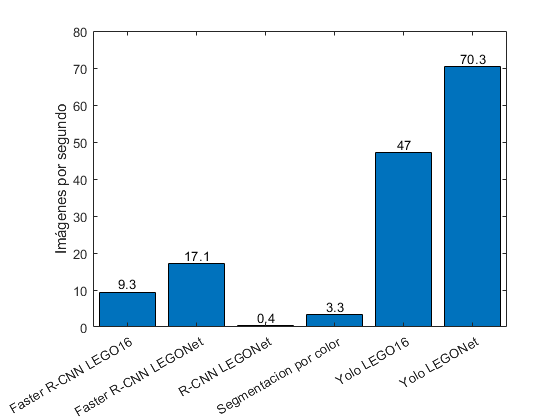
\includegraphics[width=0.95\textwidth]{Resultados/detectores barras.png}
	\caption{Diagrama de barras: Comparación de la velocidad de diferentes métodos para la segmentación (más alto es mejor)}
	\label{fig:velocidad barras}
\end{figure}

\begin{figure}[ht]  %Cajas velicadad
	\centering
	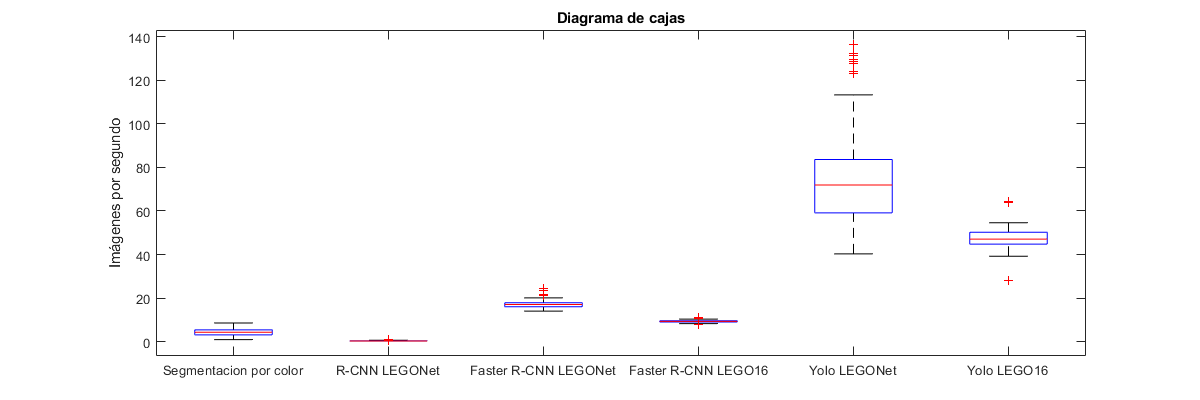
\includegraphics[width=0.95\textwidth]{Resultados/detectores cajas.png}
	\caption{Diagrama de cajas: Comparación de la velocidad de diferentes métodos para la segmentación (más alto es mejor)}
	\label{fig:velocidad cajas}
\end{figure}

\newpage
\section{Análisis del cálculo de la orientación}
En este proyecto también se han desarrollado múltiples métodos para el cálculo de la orientación es por ello que en esta sección se van a mostrar y comparar los resultados de los tres métodos.

\subsection{Precisión}
Los tres métodos destacan por ofrecer buenos resultados, aunque hay un método claramente superior al resto. A continuación, se muestran los resultados de los tres métodos para su comparación.

\begin{itemize}
\item Transformada de Hough: Se observa que es un método bastante preciso ya que el eror medio no es elevado. Sin embargo, no es un método robusto ya que hay varias situaciones donde el error cometido el demasiado grande.
\item LEGONet: Este método es el que mejor resultados ha dado con un error prácticamente nulo y una robustez clara. Demuestra el claro potencial de las redes neuronales.
\item LEGO16: Este método ha dado resultados también bastante precisos, aunque ha cometido varios errores demasiado grandes y por ello falla en robustez. Se cree que esta red no ha sido bien diseñada o entrenada y que tiene un potencial mayor al mostrado.
\end{itemize}

\begin{table}[ht] %tabla orientación precision
  \centering
    \begin{tabular}{|l|r|r|r|}
    \cline{2-4} \multicolumn{1}{r|}{} & \multicolumn{1}{l|}{Transformada de Hough} & \multicolumn{1}{l|}{LEGONet} & \multicolumn{1}{l|}{LEGO16}\\	
    \hline
    Error medio & 0.98$^{\circ}$  & 0.33$^{\circ}$ & 0.71$^{\circ}$ \\
    \hline
    Error máximo & 26$^{\circ}$  & 1.3$^{\circ}$ & 16$^{\circ}$ \\
    \hline
    Precisión & 83.67\% & 97.67\% & 79.33\% \\
    \hline
    Desviación típica & 1.82$^{\circ}$ & 0.43$^{\circ}$ & 1.23$^{\circ}$ \\
    \hline
    \end{tabular}%
  \label{tab:oreintacion precision cajas}%
  \caption{Comparación del error medio, error máximo, precisión y desviación típica de diferentes métodos para el cálculo de la orientación}
\end{table}

\begin{figure}[ht]  %Cajas orientación precision
	\centering
	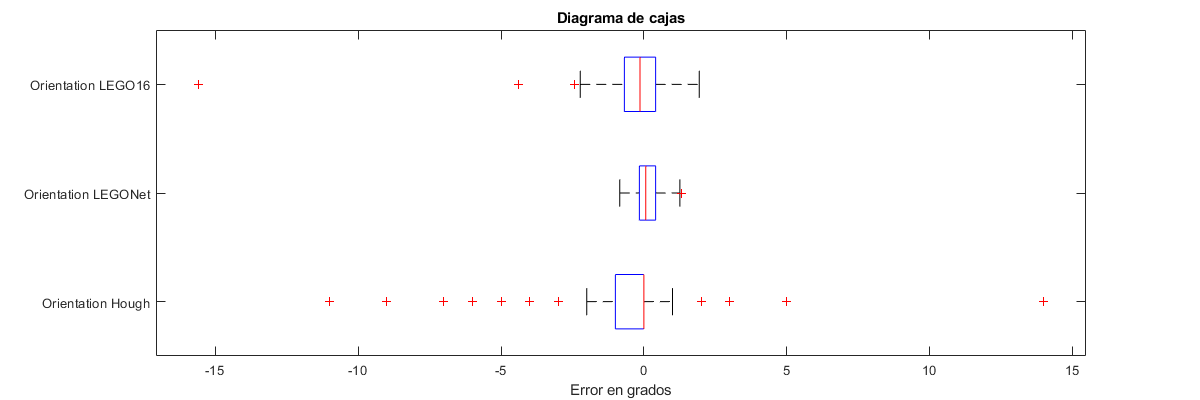
\includegraphics[width=0.95\textwidth]{Resultados/orientacion precision cajas.png}
	\caption{Diagrama de cajas: Comparación de la precisión de diferentes métodos para el cálculo de la orientación (cuanto más centrado respecto al cero y menos disperso mejor)}
	\label{fig:oreintacion precision cajas}
\end{figure}

\newpage
\subsection{Velocidad}
Al igual que con la segmentación, en este caso también se va a realizar un estudio de la velocidad de los diferentes métodos ya que esta tendrá un impacto en el rendimiento del sistema en su conjunto.

\begin{itemize}
\item Transformada de Hough: Se caracteriza por ser un método rápido y constante. El tiempo de análisis de cada pieza es muy similar y apenas hay variaciones.
\item LEGONet: Este método es el más rápido de los tres, aunque es menos constante en su rapidez. También hay que tener en cuenta, que al ir más rápido un pequeño retraso al analizar una pieza tiene un mayor impacto.
\item LEGO16: Este método ha dado resultados también bastante rápido aunque presenta numerosas situaciones en los que la velocidad ha reducido bastante.
\end{itemize}

En general los tres métodos son muy rápidos y todos han dado resultados superiores a las sesenta piezas por segundo, aunque es importante tener en cuenta que estos métodos se deben de correr tantas veces como piezas haya en la imagen.

\begin{figure}[ht]  %Barras velicadad
\vspace{-10pt}
	\centering
	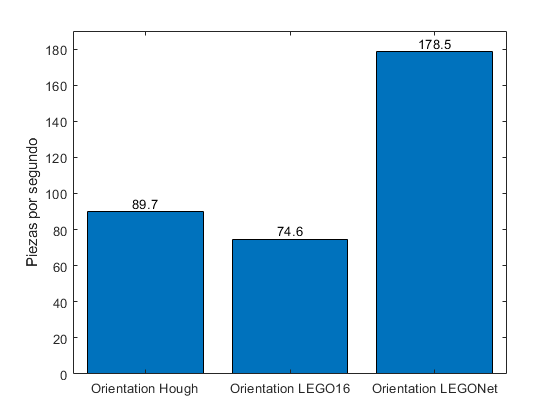
\includegraphics[width=0.7\textwidth]{Resultados/orientacion velocidad barras.png}
	\caption{Diagrama de barras: Comparación de la velocidad de diferentes métodos para el cálculo de la orientación (más alto es mejor)}
	\label{fig:orientacion velocidad barras}
\end{figure}

\begin{figure}[ht]  %Cajas velicadad
\vspace{-10pt}
	\centering
	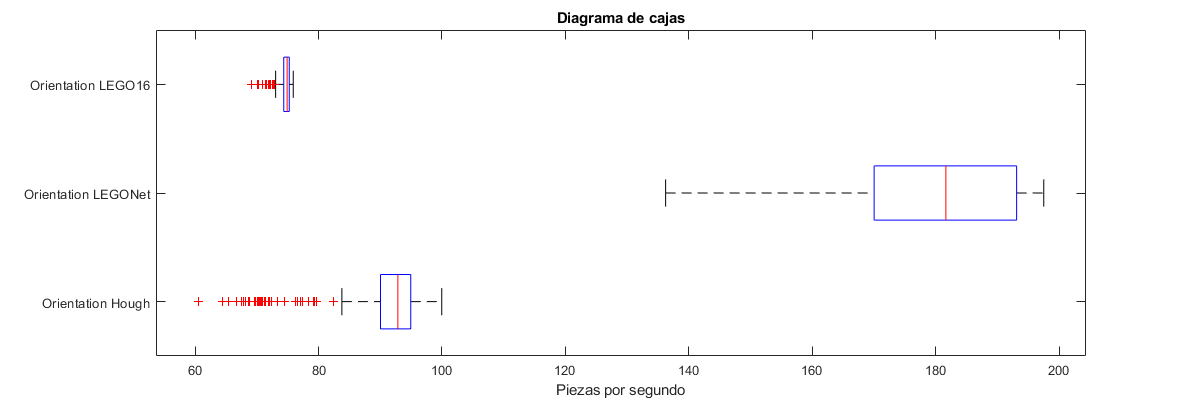
\includegraphics[width=1\textwidth]{Resultados/orientacion velocidad cajas.png}
	\caption{Diagrama de cajas: Comparación de la velocidad de diferentes métodos para el cálculo de la orientación (más a la derecha es mejor)}
	\label{fig:orientacion velocidad cajas}
\end{figure}